
%There is a bicategory $\cat{V}$ of smooth projective algebraic varieties over $\mathbb{C}$ \cite{??}, where the $1$-morphisms between varieties $\md{x}: A \lto B$ are Fourier-Mukai kernels, that is, complexes of coherent sheaves $\md{X}$ on the product $A \times B$. 

%For example, let $B = Proj(A)$ for some graded algebra $A = k[x_1,\ldots,x_n]/I$, and let $\md{X}, \md{Y}$ be complexes of vector bundles on $B$. In the bicategory $\cat{V}$ there are $1$-morphisms
%\[
%\xymatrix@C+2pc{
%\operatorname{pt} \ar[r]^-{\md{X}} & B \ar[r]^-{\md{Y}^{\vee}} & \operatorname{pt}
%}
%]
%where $\operatorname{pt} = \Spec(\mathbb{C})$. The composite in $\cat{V}$ is the complex
%\begin{equation}\label{eq:infinite_tensor_scheme}
%y^{\vee} \otimes^{\mathbb{L}} x = \md{Y}^{\vee} \otimes^{\mathbb{L}} \md{X} \cong 
%\end{equation}
%which is infinite-dimensional but has finite-dimensional cohomology. 

%Suppose that $\md{X}, \md{Y}$ are finitely described, for example that $X, Y$ are complexes of finitely generated graded free $A$-modules and $\md{X}, \md{Y}$ the associated complexes of sheaves, which are therefore described in terms of finite lists of matrices of homogeneous polynomials. 

\section{Defining Cut systems}

To complete the construction of the cut system we need to finish defining the associator and unitors (a task begun at the outset of the section) and to prove that the coherence conditions hold. 

Earlier the unitors were described by explicit formulas. Here we begin more abstractly: let $X \in \cat{L}(W,V)$ be a matrix factorisation with $W \in k[x_1,\ldots,x_n]$ and $V \in k[z_1,\ldots,z_m]$. Since $\Delta_V$ is the unit in $\LG$ there is a homotopy equivalence $\lambda: \Delta_V \otimes_{k[z]} X \lto X$ and so by Proposition \ref{prop:final_homotopy_equiv_cut} there are homotopy equivalences
\begin{equation}
\xymatrix@C+3pc{
\Delta_V \l X \ar@<-1ex>[r]_-{\Phi^{-1}} & S_m \otimes_k ( \Delta_V \otimes X )\ar@<-1ex>[l]_-{\Phi} \ar@<-1ex>[r]_-{1 \otimes \lambda} & S_m \otimes_k X \ar@<-1ex>[l]_-{1 \otimes \lambda^{-1}} 
}\,.
\end{equation}
By construction these isomorphisms are $A_m$-linear, and the map from right to left is an isomorphism $\mu: X \lto \Delta_V \l X$ in $\cat{L}(W,V)^\bullet$ corresponding under Lemma \ref{lemma:morphism_out_1} to
\[
\mu_0 = \xymatrix@C+1pc{
X \ar[r]^-{\lambda^{-1}} & \Delta_V \otimes_{k[z]} X \ar[r]^-{\varrho} & \Delta_V \l X
}\,.
\]
where $\varrho$ is the quotient map. Given the explicit formula for $\lambda^{-1}$ from \cite[Section 4.1]{lgdual}, this map $\mu_0$ has the explicit formula given earlier in \eqref{eq:explicit_mu0}. Since $\mu_0$ is natural in $X$, this also proves that $\mu$ is a natural isomorphism. The details for $\eta$ are similar, so the unitors are now defined.

The remaining components of the cut system $\cat{L}$ are the units $\Delta_W \in \cat{L}(W,W)$, which are the same as those for $\LG$ given in Section \ref{section:superbicatLG}, and the associators and unitors. 

The unitors can also be described by explicit formulas. Given $X \in \cat{L}(W,V)$ as above with homogeneous basis $e_i$ as a $\mathbb{Z}_2$-graded $k[x,z]$-module, we define morphisms of matrix factorisations
\begin{gather}
\mu_0: X \lto \Delta_V \l X \,, \\
\mu_0(e_i) = \sum_{l \ge 0} \sum_{i_1 < \cdots < i_l} \sum_j \Theta_{i_1} \ldots \Theta_{i_l} \left\{ \partial^{z,z'}_{[i_l]}(d_X) \cdots \partial^{z,z'}_{[i_1]}(d_X) \right\}_{ji} \otimes e_j\label{eq:explicit_mu0}
\end{gather}
and
\begin{gather}
\eta_0: X \lto X \l \Delta_W \,,\\
\eta_0(e_i) = \sum_{l \ge 0} \sum_{i_1 < \cdots < i_l} \sum_j (-1)^{\binom{l}{2} + l|e_i|} e_j \otimes \left\{ \partial^{x,x'}_{[i_1]}(d_X) \cdots \partial^{x,x'}_{[i_l]}(d_X) \right\}_{ji} \Theta_{i_1} \ldots \Theta_{i_l}
\end{gather}
To make sense of these formulas, note that $\Delta_V$ is a matrix factorisation of $V(z) - V(z')$ over $k[z,z']$ and $\Delta_W$ is a matrix factorisation of $W(x) - W(x')$ over $k[x,x']$, while the divided difference operators are defined by
\[
{}^{t_i}(-): k[x,x'] \lto k[x,x']\,, \qquad f \mapsto f|_{x_i \mapsto x'_i}
\]
and
\[
\partial^{x,x'}_{[i]}: k[x,x'] \lto k[x,x']\,, \qquad f \mapsto \frac{{}^{t_1 \ldots t_{i-1}} f - {}^{t_1 \ldots t_i} f}{x_i - x'_i}
\]
and in the same way for $z,z'$. For a concrete example of these formulas see \cite{lgdual_survey}. The actual unitors are the morphisms $X \lto \Delta_V \l X$ and $X \lto X \l \Delta_W$ in $\cat{L}(W,V)^\bullet$ corresponding to $\mu_0$ and $\eta_0$ under the bijection of Lemma \ref{lemma:morphism_out_1}. It is not meant to be clear \emph{a priori} that these formulas even define morphisms, let alone that they satisfy the axioms for unitors; all these checks will be performed below.

\section{Convolution as a morphism of schemes}

We either fix a basis for Jacobians or assume $k$ a field so we can use Grobner.

\begin{itemize}
\item Restate hmf as matrices
\item Do idempotent completion as matrices with chosen homotopies
\item Do Clifford thickening as matrices with chosen homotopies
\item Write down the morphism of schemes
\end{itemize}

% This is the definition from cutsys10
\begin{definition} A \emph{cut system} $\cat{A}$ is determined by the following data:
\begin{itemize}
\item A class $|\cat{A}|$ of objects and for each object $a$ an integer $\pi(a) \ge 0$.
\item For each pair $a,b$ of objects a small idempotent complete supercategory $\cat{A}(a,b)$. 
\item For each triple $a,b,c$ of objects a cut functor of degree $\pi(b)$
\[
T: \cat{A}(a,b) \otimes_k \cat{A}(b,c) \lto \cat{A}(a,c)^{\bullet}\,.
\]
The image of a pair $X \otimes Y$ under the canonical extension
\[
\widetilde{T}: \cat{A}(a,b)^\bullet \otimes_k \cat{A}(b,c)^\bullet \lto \cat{A}(a,c)^\bullet
\]
is denoted $Y \l X$ and is called the \emph{cut of $Y$ and $X$ along $b$}.
\item For each object $a$, an object $\Delta_a \in \cat{A}(a,a)$.
\item For objects $a,b,c,d$ a natural isomorphism $\alpha$ as shown below:
\[
\xymatrix@C+2pc{
\cat{A}(a,b) \times \cat{A}(b,c) \times \cat{A}(c,d) \ar[d]_-{T \times 1} \ar[r]^-{1 \times T} & \cat{A}(a,b) \times \cat{A}(b,d)^\bullet \ar[d]^{\widetilde{T}} \ar@{=>}[dl]^-{\alpha}\\
\cat{A}(a,c)^\bullet \times \cat{A}(c,d) \ar[r]_-{\widetilde{T}} & \cat{A}(a,d)^\bullet
}
\]
That is, for $X \in \cat{A}(a,b), Y \in \cat{A}(b,c), Z \in \cat{A}(c,d)$ an isomorphism
\[
\alpha_{Z,Y,X}: ( Z \l Y ) \l X \lto Z \l ( Y \l X )
\]
of $A_{\pi(b)} \otimes_k A_{\pi(c)}$-modules in $\cat{A}(a,d)$, natural in all three variables.
\item For objects $a,b$ natural isomorphisms $\mu, \eta$ as shown below:
\[
\xymatrix@C+2pc{
1 \times \cat{A}(a,b) \ar[d]_-{\iota_{\Delta} \times 1} & \cat{A}(a,b) \ar@{=>}@<4ex>[l]_-{\eta} \ar@{=>}@<-4ex>[r]^-{\mu} \ar[d]^-{\iota} \ar[l]_-{\cong} \ar[r]^-{\cong} & \cat{A}(a,b) \times 1 \ar[d]^-{1 \times \iota_{\Delta}}\\
\cat{A}(a,a) \times \cat{A}(a,b) \ar[r]_-{T} & \cat{A}(A,B)^\bullet & \cat{A}(a,b) \times \cat{A}(b,b) \ar[l]^-{T}
}
\]
where $1$ is the category with one object and one morphism and $\iota_{\Delta}$ is the functor sending this object to $\Delta$. That is, for each $X \in \cat{A}(a,b)$ a pair of isomorphisms
\begin{equation}\label{eq:defn_cutsys_lambda}
\mu: X \lto \Delta_b \l X, \quad \eta: X \lto X \l \Delta_a
\end{equation}
in $\cat{A}(a,b)^\bullet$ natural in $X$.
\end{itemize}
This data is subject to the following coherence conditions:
\begin{itemize}
\item[(1)] For objects $a,b,c,d,e$ and $X \in \cat{A}(a,b),Y \in \cat{A}(b,c),Z \in \cat{A}(c,d),Q \in \cat{A}(d,e)$, commutativity of the diagram
\begin{equation}
\xymatrix@C+2pc{
((Q \l Z) \l Y ) \l X \ar[d]_-{\alpha_{Q \l Z, Y, X}}\ar[r]^-{\alpha_{Q,Z,Y} \l 1} & (Q \l (Z \l Y)) \l X \ar[r]^-{\alpha_{Q, Z \l Y, X}} & Q \l ( ( Z \l Y ) \l X ) \ar[d]^-{1 \l \alpha_{Z,Y,X}}\\
(Q \l Z) \l (Y \l X) \ar[rr]_-{\alpha_{Q, Z, Y \l X}} & & Q \l ( Z \l ( Y \l X ) )
}
\end{equation}
Note that when we write $\alpha_{Q, Z \l Y, X}$ we refer only the underlying object of $Z \l Y$.
\item[(2)] For objects $a,b$ and $X \in \cat{A}(a,b), Y \in \cat{A}(b,c)$ commutativity of the diagram
\begin{equation}\label{eq:unitor_constraint_cut}
\xymatrix{
(Y \l \Delta_b ) \l X \ar[rr]^-{\alpha} & & Y \l ( \Delta_b \l X )\\
& Y \l X \ar[ul]^-{\eta \l 1_X} \ar[ur]_-{1_Y \l \mu}
}
\end{equation}
\item[(3)] commutativity of \eqref{eq:psiunitor1},\eqref{eq:psiunitor2} for every $X$ and \eqref{eq:psithirdlastdia}, \eqref{eq:psimiddledia}, \eqref{eq:psilastdia} for every composable triple $X,Y,Z$.
\end{itemize}
%Finally, the data is subject to three computability conditions:
%\begin{itemize}
%\item[(1)] For each pair of objects $a,b$ the category $\cat{A}(a,b)$ is effectively computable, in the sense that the morphisms and objects are described by finite data and the composition rule is computable.
%\item[(2)] For each triple $a,b,c$ of objects the associated cut functor is effectively computable. In particular, for $1$-morphisms $Y$ and $X$ the object $Y \l X$ and its Clifford action are effectively computable from $X$ and $Y$.
%\item[(3)] The associators and unitors are effectively computable from their arguments.
%\end{itemize}
\end{definition}

Let $\cat{A}$ be a cut system. There is a superbicategory $\cat{A}^\bullet$ with objects the class of objects of $\cat{A}$ and with $1$- and $2$-morphisms defined by $\cat{A}^\bullet(a,b) = \cat{A}(a,b)^\bullet$. The units of $\cat{A}^\bullet$ are the objects $\Delta_a$ in the cut system, and the composition in the bicategory is given by the canonical extensions $\widetilde{T}$. To complete the definition of a superbicategory it only remains to give the associators and unitors, and the super-structure.

\begin{lemma} Given objects $a,b,c,d$ the natural isomorphism $\alpha$ canonically extends to a natural isomorphism $\widetilde{\alpha}$ as in the diagram
\[
\xymatrix@C+2pc{
\cat{A}(a,b)^\bullet \times \cat{A}(b,c)^\bullet \times \cat{A}(c,d)^\bullet \ar[d]_-{\widetilde{T} \times 1} \ar[r]^-{1 \times \widetilde{T}} & \cat{A}(a,b)^\bullet \times \cat{A}(b,d)^\bullet \ar[d]^{\widetilde{T}} \ar@{=>}[dl]^-{\widetilde{\alpha}}\\
\cat{A}(a,c)^\bullet \times \cat{A}(c,d)^\bullet \ar[r]_-{\widetilde{T}} & \cat{A}(a,d)^\bullet
}
\]
\end{lemma}
\begin{proof}
Suppose $(X,n) \in \cat{A}(a,b)^\bullet, (Y,m) \in \cat{A}(b,c)^\bullet$ and $(Z,t) \in \cat{A}(c,d)^\bullet$ are given. The underlying object of $((Z,t) \l (Y, m)) \l (X,n)$ is $(Z \l Y) \l X$, and it is clear that $\alpha_{Z,Y,X}$ is $A_t \otimes A_m \otimes A_n$-linear and therefore defines an isomorphism in $\cat{A}(a,d)^\bullet$
\[
\alpha_{Z,Y,X}: ((Z,t) \l (Y, m)) \l (X,n) \lto (Z,t) \l ((Y, m) \l (X,n))\,.
\]
Naturality is straightforward.
\end{proof}

\begin{lemma} Given objects $a,b$ the natural isomorphisms $\eta, \mu$ canonically extend to natural isomorphisms $\widetilde{\eta}, \widetilde{\mu}$ as in the diagram
\[
\xymatrix@C+2pc{
1 \times \cat{A}(a,b)^\bullet \ar[d]_-{\iota_{\Delta} \times 1} & \cat{A}(a,b)^\bullet \ar@{=>}@<4ex>[l]_-{\widetilde{\eta}} \ar@{=>}@<-4ex>[r]^-{\widetilde{\mu}} \ar[d]^-{1} \ar[l]_-{\cong} \ar[r]^-{\cong} & \cat{A}(a,b)^\bullet \times 1 \ar[d]^-{1 \times \iota_{\Delta}}\\
\cat{A}(a,a)^\bullet \times \cat{A}(a,b)^\bullet \ar[r]_-{\widetilde{T}} & \cat{A}(A,B)^\bullet & \cat{A}(a,b)^\bullet \times \cat{A}(b,b)^\bullet \ar[l]^-{\widetilde{T}}
}
\]
 \end{lemma}
\begin{proof}
Let $(X,n) \in \cat{A}(a,b)^\bullet$. Forgetting the $A_n$-action on $X$, we have isomorphisms $\eta$ and $\mu$ as in \eqref{eq:unitor_tilde_pre}, which are respectively $A_{\pi(b)}$ and $A_{\pi(a)}$-linear. Since these isomorphisms are natural, they are automatically $A_n$-linear. Verifying that these isomorphisms are natural with respect to the larger class of morphisms in $\cat{A}(a,b)^\bullet$ is straightforward.
\end{proof}

The supercategory structure is given as part of the cut system, so we have:

% The above definition of a cut system is from cutsys10. This is by p.11 there something which gives rise to a cut system in the sense of cutsys6, which is proved there to define a superbicategory.
\begin{proposition} Given a cut system $\cat{A}$, $\cat{A}^\bullet$ is a superbicategory.
\end{proposition}
\begin{proof}
This follows from Lemma \ref{lemma:constructingsuper}, with associator $\widetilde{\alpha}$ and unitors $\lambda =\widetilde{\mu}^{-1}, \rho = \widetilde{\eta}^{-1}$. The coherence follows from the coherence axioms of the cut system.
\end{proof}

We often confuse a cut system $\cat{A}$ with the associated superbicategory. For example, we refer to objects $X$ of $\cat{A}(a,b)^\bullet$ as a $1$-morphisms. To distinguish objects of the original category $\cat{A}(a,b)$ we refer to these objects as \emph{normal} or \emph{cut-free} $1$-morphisms. We keep the notation $Y \l X$ for the composition rule in $\cat{A}^\bullet$.

The following lemma is useful in verifying the unitor constraint.

\begin{lemma}\label{lemma:unitor_check_help} The commutativity of \eqref{eq:unitor_constraint_cut} is equivalent to commutativity of
\begin{equation}\label{eq:unitor_check_help1}
\xymatrix@C+1pc{
(Y \l \Delta_b) \l X \ar[rr]^-{\alpha} & & Y \l ( \Delta_b \l X )\\
Y \l X \ar[u]^-{\eta_0 \l 1} & Y \l X \ar[l]^-{e_{\pi(b)}} \ar[r]_-{e_{\pi(b)}} & Y \l X \ar[u]_-{1 \l \mu_0}
}
\end{equation}
where $e_{\pi(b)}$ is the idempotent of Definition \ref{defn:idempotent_e}.
\end{lemma}
\begin{proof}
Let $m = \pi(b)$. Then $(Y \l \Delta_b) \l X$ has two $A_m$ actions, one from $Y \l \Delta_b$ which we denote by $A_{m_1}$, and the other from the cut with $X$ which we denote by $A_{m_2}$. By definition of the canonical extension $\widetilde{T}$ in Appendix \ref{app:proof_cut_extension}, $\eta \l 1$ is the $A_{m_1+m_2}$-linear morphism
\[
\eta: S_{m_1 + m_2, m_2} \otimes_{A_{m_2}} ( Y \l X ) \lto (Y \l \Delta_b ) \l X
\]
which corresponds under Lemma \ref{lemma:morphisms_two_forms} to
\[
\xymatrix@C+1pc{
Y \l X \ar[r]^-{e_m} & Y \l X \ar[r]^-{\eta_0 \l 1} & (Y \l \Delta_b) \l X
}\,.
\]
Applying the same logic to $\mu$ completes the proof.
\end{proof}

In a cut system the unitors $\mu, \eta$ go in the opposite direction to what one would expect from the conventions of bicategories. This is because it is more natural to describe morphisms out of a cut-free $1$-morphism and into a $1$-morphism carrying a nontrivial Clifford representation, than in the other direction.

\begin{proof}[Proof of Theorem \ref{theorem:l_cut_system}] We first check the coherence axioms. The first and third are trivial. To prove (2) we need by Lemma \ref{lemma:unitor_check_help} only check commutativity of \eqref{eq:unitor_check_help1} in the usual situation of $X: W \lto V$ and $Y: V \lto U$. 

This amounts to checking commutativity of
\begin{equation}\label{eq:coherence3_1}
\xymatrix{
(Y \l \Delta_V ) \l X \ar[rr]^-{\alpha} & & Y \l ( \Delta_V \l X )\\
(Y \otimes \Delta_V) \otimes J_V \otimes X \ar[u]^-{\varrho \otimes 1} & & Y \otimes J_V \otimes ( \Delta_V \otimes X) \ar[u]_-{1 \otimes \varrho}\\
Y \otimes J_V \otimes X \ar[u]^-{ \rho^{-1} \otimes 1} & Y \otimes J_V \otimes X \ar[l]^-{e_m} \ar[r]_-{e_m} & Y \otimes J_V \otimes X \ar[u]_-{1 \otimes \lambda^{-1}}
}\,.
\end{equation}
By definition $e_m$ factors as
\[
\xymatrix{
Y \l X \ar[r]^-{\Phi^{-1}} & S_m \otimes_k ( Y \otimes X ) \ar[r] & Y \otimes X \ar[r] & S_m \otimes_k (Y \otimes X) \ar[r]^-{\Phi} & Y \l X
}
\]
so commutativity of \eqref{eq:coherence3_1} follows from commutativity of
\[
\xymatrix@C-0.5pc{
(Y \l \Delta_V ) \l X \ar[rrr]^-{\alpha} & & & Y \l ( \Delta_V \l X )\\
(Y \otimes \Delta_V) \otimes J_V \otimes X \ar[u]^-{\varrho \otimes 1} & (Y \otimes \Delta_V ) \otimes X \ar[l]_-{\varrho} \ar[r]^-{\alpha} & Y \otimes (\Delta_V \otimes X) \ar[r]^-{\varrho} & Y \otimes J_V \otimes ( \Delta_V \otimes X) \ar[u]_-{1 \otimes \varrho}\\
Y \otimes J_V \otimes X \ar[u]^-{ \rho^{-1} \otimes 1} & Y \otimes X \ar[u]^-{\rho^{-1} \otimes 1} \ar@{=}[r] \ar[l]^-{\varrho} & Y \otimes X \ar[u]_-{1 \otimes \lambda^{-1}} \ar[r]_-{\varrho} & Y \otimes J_V \otimes X \ar[u]_-{1 \otimes \lambda^{-1}}
}\,.
\]
The innermost square of this diagram is the coherence constraint for the unitors in $\LG$.

%Finally, we check the computability conditions. The associator and unitors are derived explicitly from $d_X$ and $d_Y$, so (3) is clear, and (2) is addressed by Remark \ref{remark:inflation} and the explicit formulas for the Clifford action. For (1), the objects and morphisms of $\cat{L}(W,V)$ are described by finite matrices of polynomials, and the composition rule is given by multiplication of matrices. There is one subtlety: morphisms are matrices of polynomials \emph{identified up to homotopy}. 

%To argue that $\cat{L}(W,V)$ is effectively computable we need to show that it is possible to determine algorithmically whether two morphisms are homotopic. This is important even at the level of objects: an object is a pair $(X,e)$ where $e^2 = e$ holds up to homotopy. Without an effective homotopy relation, there would be no algorithmic way to even distinguish between objects and non-objects. The necessary check is in Section \ref{example:computing_homs}.
\end{proof}

We will use \emph{effectively computable} as a synonym for the precise notion of a \emph{computable} function \cite{enderton}, since ``computable'' often has a more colloquial meaning in our context.



\begin{remark} To give natural isomorphisms \eqref{eq:defn_cutsys_lambda} in $\cat{A}(a,b)^\bullet$ is equivalent to giving natural isomorphisms in $\cat{A}(a,b)$
\begin{equation}\label{eq:unitor_tilde_pre}
\mu: S_{\pi(b)} \otimes_k X \lto \Delta_b \l X, \quad \eta: S_{\pi(a)} \otimes_k X \lto X \l \Delta_a
\end{equation}
which are respectively $A_{\pi(b)}$ and $A_{\pi(a)}$-linear. 

By Lemma \ref{lemma:morphism_out_1} such morphisms correspond bijectively to morphisms in $\cat{A}(a,b)$
\begin{equation}\label{eq:unitor_tilde}
\mu_0: X \lto \Delta_b \l X, \quad \eta_0: X \lto X \l \Delta_a
\end{equation}
satisfying respectively $a_i^\dagger \circ \mu_0 = 0$ for $1 \le i \le m$ and $a_i^\dagger \circ \eta_0 = 0$ for $1 \le i \le n$. The reason to introduce these maps is that commutativity of \eqref{eq:unitor_constraint_cut} can be more conveniently expressed in terms of the maps in \eqref{eq:unitor_tilde}, see Lemma \ref{lemma:unitor_check_help} below.
\end{remark}

\subsection{Cut models}\label{section:cut_models}

\begin{definition} A \emph{cut model} for a superbicategory $\cat{B}$ is a cut system $\cat{A}$ with the same underlying class of objects as $\cat{B}$ and a strong superfunctor $I: \cat{B} \lto \cat{A}^\bullet$ with the property that for every pair of objects $a,b$ the functor
\[
I_{a,b}: \cat{B}(a,b) \lto \cat{A}(a,b)^\bullet
\]
factors as
\[
\xymatrix{
\cat{B}(a,b) \ar[rr]^-{I_{a,b}} \ar[dr]_-{J_{a,b}} & & \cat{A}(a,b)^\bullet\\
& \cat{A}(a,b) \ar[ur]_-{\iota}
}
\]
where $J_{a,b}$ is an equivalence of supercategories. We often identify $X$ with $I(X)$.
\end{definition}

A cut model is an effectively computable model for composition of $1$-morphisms in~$\cat{B}$. Given $X: a \lto b$ and $Y: b \lto c$, let us suppose that the composition $Y \circ X$ in $\cat{B}$ is not defined algorithmically: perhaps this object is only identified up to unique isomorphism by a universal property. In contrast, the cut $Y \l X$ is computable from $X$ and $Y$, and the strong superfunctor $I$ provides an isomorphism in $\cat{A}(a,c)^\bullet$
\begin{equation}
Y \l X \cong Y \circ X\,.
\end{equation}
Here $Y \circ X$ is embedded into $\cat{A}^\bullet$ as a cut-free $1$-morphism and the cut $Y \l X$ by definition comes with an $A_{\pi(b)}$-module structure. That is, there is an isomorphism of $A_{\pi(b)}$-modules
\begin{equation}\label{eq:cutvsoriginal}
Y \l X \cong S_{\pi(b)} \otimes_k (Y \circ X )
\end{equation}
or what is the same, an isomorphism of objects in $\cat{A}(a,b)$
\begin{equation}\label{eq:cutvsoriginal2}
S^*_{\pi(b)} \otimes_{A_{\pi(b)}} ( Y \l X ) \cong Y \circ X \,.
\end{equation}
The general philosophy is that a cut model decomposes composition in $\cat{B}$ into two stages: 
\begin{itemize}
\item first form the cut $Y \l X$, and then
\item tensor $Y \l X$ with $S^*_{\pi(b)}$ to compute $Y \circ X$. 
\end{itemize}
The idea is that the desired composition $Y \circ X$ lies inside $Y \l X$ in a way that is ``known'' in the sense that it is encoded by the Clifford action, but which is only \emph{realised} or \emph{constructed} after a computation is done. Forming the tensor product $S^*_{\pi(b)} \otimes_{A_{\pi(b)}} ( Y \l X )$ starting with the concretely known object $Y \l X$ can be further decomposed into a $\pi(b)$-step process of ``atomic'' computations, using the diagram of Remark \ref{remark:tensor_and_idempotent}
\begin{equation}\label{eq:computation_fiber_diagram}
\xymatrix@C+1pc@R+1pc{
Z_0 \cong Y \circ X \ar@{.}[d] & Z_1 \ar@{.}[d] & & Z_{\pi(b)-1} \ar@{.}[d] & Z_{\pi(b)} = Y \l X \ar@{.}[d]\\
0 \ar@{.>}@<0.8ex>[r] & 1 \ar@{.>}@<0.8ex>[r]\ar@{.>}@<0.8ex>[l] & \cdots \ar@{.>}@<0.8ex>[l]\ar@{.>}@<0.8ex>[r] & \pi(b)-1  \ar@{.>}@<0.8ex>[l]\ar@{.>}@<0.8ex>[r] & \pi(b) \ar@{.>}@<0.8ex>[l]
}\,.
\end{equation}
% remark:tensor_in_steps.
The intermediate objects are $Z_i = S_{i, \pi(b)} \otimes_{A_{\pi(b)}} ( Y \l X )$ for $i < \pi(b)$. Each of these objects $Z_i$ is obtained from $Z_{i+1}$ by splitting an idempotent of the form $a^\dagger a$.

Suppose we are in the situation where $Y \circ X$ is identified by a universal property but an explicit object realising this universal property is not given as part of $\cat{B}$. Then the result of the $\pi(b)$-step computation depicted above is an explicit object $Z_0$ of $\cat{A}(a,c) \cong \cat{B}(a,c)$ with this universal property. Thus the cut system gives a process for constructing representing objects for the uniquely defined isomorphism class $Y \circ X$ of $\cat{B}(a,c)$.

Conceptually, the number of steps in \eqref{eq:computation_fiber_diagram} represents the computational cost of a cut across the object $b$. For any cut across this object, $\pi(b)$-steps are necessary to convert the ``uncertainty'' represented by $Y \l X$ with its $A_{\pi(b)}$-action to the certainty of an object of $\cat{A}(a,c)$ (in the sense of Remark \ref{remark:tensor_and_idempotent}). In the example of the next section, the cost $\pi(W)$ of cutting across a hypersurface singularity $W$ is determined by its dimension.

\section{Cut systems}\label{section:cut_systems}

We begin with the definition of cut functors.

\begin{definition} Given supercategories $\cat{C}_1,\cat{C}_2,\cat{C}_3$ a \emph{superfunctor} $T: \cat{C}_1 \otimes_k \cat{C}_2 \lto \cat{C}_3$ is a functor together with natural isomorphisms
\begin{align*}
\tau &: T \circ ( \Psi \otimes 1 ) \lto \Psi \circ T,\\
\tau &: T \circ ( 1 \otimes \Psi ) \lto \Psi \circ T
\end{align*}
making the following diagrams commute:
\begin{equation}\label{eq:psicomp1}
\xymatrix@R+1pc@C+1pc{
T( 1 \otimes \Psi^2 ) \ar[r]^-{\tau}\ar[d]_-{T(1 \otimes \xi)} & \Psi T( 1 \otimes \Psi ) \ar[r]^-{\tau} & \Psi^2 T \ar[d]^-{\xi * 1_T}\\
T \ar[rr]_-{1_T} & & T
}
\end{equation}
\begin{equation}\label{eq:psicomp2}
\xymatrix@R+1pc@C+1pc{
T( \Psi^2 \otimes 1 ) \ar[r]^-{\tau} \ar[d]_-{T (\psi \otimes 1)}  & \Psi T( \Psi \otimes 1 ) \ar[r]^-{\tau} & \Psi^2 T \ar[d]^-{\xi * 1_T}\\
T \ar[rr]_-{1_T} & & T
}
\end{equation}
\begin{equation}\label{eq:psicomp3}
\xymatrix@R+1pc@C+1pc{
T( \Psi \otimes \Psi ) \ar[r]^-{\tau}\ar[d]_-{-\tau} & \Psi T( 1 \otimes \Psi ) \ar[d]^-{\tau}\\
\Psi T( \Psi \otimes 1 ) \ar[r]_-{\tau} & \Psi^2 T
}
\end{equation}

\end{definition}

\begin{definition}\label{defn:cutfunctor1} A \emph{cut functor of degree $t$} on a triple $\cat{C}_1, \cat{C}_2,\cat{C}_3$ of idempotent complete small supercategories is a superfunctor $T: \cat{C}_1 \otimes_k \cat{C}_2 \lto \cat{C}_3^\bullet$ such that
\[
\xymatrix{
\cat{C}_1 \times \cat{C}_2 \ar[r]^-{T} & \cat{C}_3^\bullet \ar[r]^-{p} & \mathbb{N}
}
\]
sends every object to the integer $t \in \mathbb{N}$.
\end{definition}

With the above notation:

\begin{proposition}\label{prop:extend_cut_functor} Given a cut functor $T$ of degree $t$ on $\cat{C}_1, \cat{C}_2,\cat{C}_3$ there is a canonical superfunctor $\widetilde{T}: \cat{C}_1^\bullet \otimes_k \cat{C}_2^\bullet \lto \cat{C}_3^\bullet$ with the property that the diagram
\[
\xymatrix{
\cat{C}_1 \times \cat{C}_2 \ar[dr]_-{\iota \times \iota} \ar[rr]^-{T} & & \cat{C}_3^\bullet\\
& \cat{C}_1^\bullet \times \cat{C}_2^\bullet \ar[ur]_-{\widetilde{T}}
}
\]
commutes, and for every pair of objects $X \in \cat{C}_1^\bullet$ and $Y \in \cat{C}_2^\bullet$
\[
p \widetilde{T}( X, Y ) = p( X ) + p( Y ) + t\,.
\]
We refer to $\widetilde{T}$ as the \emph{extension} of $T$.
%and
%\[
%\xymatrix@C+2pc{
%\cat{C}_1^\bullet \times \cat{C}_2^\bullet \ar[d]_-{p \times p}\ar[rr]^-{\widetilde{T}} & & \cat{C}_3^\bullet \ar[dd]^-{p}\\
%\mathbb{N} \times \mathbb{N} \ar[d]_-{\cong}\\
%\mathbb{N} \times \{ * \} \times \mathbb{N} \ar[r]_-{1 \times t \times 1} & \mathbb{N} \times \mathbb{N} \times \mathbb{N} \ar[r]_-{\otimes} & \mathbb{N}
%}
%\]
%commute. 
\end{proposition}
\begin{proof}
The proof is given in Appendix \ref{app:proof_cut_extension}.
\end{proof}

\section{Extending cut functors}\label{app:proof_cut_extension}

The purpose of this appendix is to give the proof of Proposition \ref{prop:extend_cut_functor}. First, note that

\begin{lemma}\label{lemma:altcomppersp} Let $\cat{C}$ be a small idempotent complete supercategory and take morphisms
\[
\xymatrix{
(X,n) \ar[r]^-{\alpha} & (Y,m) \ar[r]^-{\beta} & (Z,l)
}\\
\]
in $\cat{C}^\bullet$. Under \eqref{eq:isodefatensor} these correspond to bimodule maps
\[
\widetilde{\alpha}: S_{m,n} \lto \cat{C}^*(X,Y)\,, \qquad \widetilde{\beta}: S_{l,m} \lto \cat{C}^*(Y,Z)\,.
\]
The composite $\beta \circ \alpha: S_{l,n} \otimes_{A_n} X \lto Z$ in $\cat{C}^\bullet$ corresponds to the composite
\[
\xymatrix{
S_{l,n} \cong S_{l,m} \otimes_{A_m} S_{m,n} \ar[r]^-{\widetilde{\beta} \otimes \widetilde{\alpha}} & \cat{C}^*(Y,Z) \otimes_{A_m} \cat{C}^*(X,Y) \ar[r]^-{\circ} & \cat{C}^*(X,Z)
}\,.
\]
\end{lemma}
\begin{proof}
Follows by evaluation on $1 \otimes 1^* \in S_{l,n}$.
\end{proof}

\begin{proof}[Proof of Proposition \ref{prop:extend_cut_functor}]
Given $(X,n) \in \cat{C}_1^\bullet$ and $(Y,m) \in \cat{C}_2^\bullet$ we have $T(X,Y) = (Z,t)$ for some object $Z$ of $\cat{C}_3$. Given $a \in A_n$, say of odd degree, there is a morphism of $A_t$-modules $Z \lto \Psi Z$ given by
\[
\xymatrix@C+2pc{
T(X,Y) \ar[r]^-{T(a \otimes 1)} & T(\Psi X, Y ) \ar[r]^-{\tau} & \Psi T(X,Y)
}
\]
and this defines an algebra morphism $A_n \lto \cat{C}_3^*(Z,Z)$. Doing the same for $A_m$ defines a morphism $A_{m+t+n} \cong A_m \otimes A_t \otimes A_n \lto \cat{C}_3^*(Z,Z)$ and an object $(Z, m + t +n) \in \cat{C}_3^\bullet$. We define $\widetilde{T}$ on objects by
\begin{equation}\label{eq:ttilde}
\widetilde{T}( (X,n), (Y,m) ) = (Z, m + t + n)\,.
\end{equation}
Next we define $\widetilde{T}$ on morphisms. Given $\alpha: (X_1,n_1) \lto (X_2,n_2)$ in $\cat{C}_1^\bullet$ and $T(X_i,Y) = (Z_i,t)$ for $i = 1,2$ we must construct a morphism
\[
\widetilde{T}(\alpha,1): (Z_1, m+t+n_1) \lto (Z_2, m+t+n_2)\,.
\]
Since $\alpha$ corresponds to an $A_{n_1}$-linear map $\widetilde{\alpha}: V \lto \cat{C}_1^*(X_1,X_2)$ we can compose with $T$ to get an $A_{n_2}$-$A_{n_1}$-bilinear map $\eta := T(1,Y) \circ \widetilde{\alpha}: V \lto \cat{C}_3^*(Z_1,Z_2)$. This extends to a morphism of $A_{n_2+c}$-$A_{n_1+c}$-bimodules
\[
V \otimes_k A_c \lto \cat{C}_3^*(Z_1,Z_2), \qquad v \otimes a \mapsto \eta(v) a\,.
\]
There is a canonical isomorphism of $A_{n+2+c}$-$A_{n_1+c}$-bimodules
\begin{align*}
S_{n_2+c,n_1+c} \cong S_{n_2+c} \otimes_k S_{n_1+c}^* \cong (S_{n_2} \otimes_k S_c) \otimes_k (S_c^* \otimes_k S_{n_1}^*) \cong V \otimes_k (S_c \otimes_k S_c^*) \cong V \otimes_k A_c
\end{align*}
so we have constructed $S_{n_2+c,n_1+c} \lto \cat{C}_3^*(Z_1,Z_2)$ which corresponds to a morphism of $A_{n_2+c}$-modules $S_{n_2+c, n_1+c} \otimes_{A_{n_1+c}} Z_1 \lto Z_2$ which we define to be $\widetilde{T}(\alpha,1)$. Functoriality of this construction follows from Lemma \ref{lemma:altcomppersp}. The functoriality in the other variable follows similarly. By construction $\widetilde{T}$ makes both of the required diagrams commute.
\end{proof}

\subsection{The cut model of $\LG$}

Let $\cat{L}$ be the cut system described above, and let $\cat{L}^\bullet$ denote the associated superbicategory. With $\LG$ the superbicategory of Section \ref{section:superbicatLG} we construct a cut model $I: \LG \lto \cat{L}^\bullet$. On objects $I$ is the identity. For potentials $V,W$ we need to define a functor
\begin{equation}\label{eq:cut_model_equiv}
I_{V,W}: \LG(W,V) \lto \cat{L}^\bullet(W,V)\,.
\end{equation}
Recall that with $\cat{C} = \hmf(k[x,z], V - W)$,
\[
\cat{L}^\bullet(W,V) = \cat{C}^{\omega \bullet}\,, \quad \LG(W,V) = \cat{C}^{\oplus}\,.
\]
An object of $\cat{C}^{\omega \bullet}$ is a tuple $((X,e), n)$ consisting of an integer $n \ge 0$ and an $A_n$-module $(X,e)$ in $\cat{C}^\omega$, while an object of $\cat{C}^{\oplus}$ is a (possibly infinite) matrix factorisation of $V - W$ which is a direct summand of a finite rank one.

On the full subcategory of finite rank matrix factorisation of $V - W$, $I_{V,W}$ is the identity and this functor extends uniquely (up to natural equivalence) to $\LG(W,V)$. To be more explicit about it: for each $X \in \LG(W,V)$ we \emph{choose} a finite rank matrix factorisation $\bar{X}$ together with an idempotent $e$ and morphisms $f_X, g_X$ as in the diagram
\[
\xymatrix@C+2pc{
\bar{X} \ar@(ul,dl)_-{e} \ar@<1ex>[r]^-{f_X} & X \ar@<1ex>[l]^-{g_X}
}
\]
satisfying $g_X f_X = e$ and $f_X g_X = 1_X$. Then the full definition of $I$ is given by
\[
I( X ) = ((\bar{X}, e), 0)\,, \qquad I( \phi ) = g_Y \phi f_X\,.
\]
To complete the definition of a strong functor $I$ it remains to give a natural $2$-isomorphism
\begin{equation}\label{eq:strong_functor_varphi}
\varphi: I(Y \otimes X) \lto I(Y) \l I(X)
\end{equation}
for every pair of $1$-morphisms $X: W \lto V$ and $Y: V \lto U$ in $\LG$. 

We give the definition of $\varphi$ where $X,Y$ are finite rank matrix factorisations; the general case follows. Recall the $A_m$-linear isomorphism of Proposition \ref{prop:final_homotopy_equiv_cut}
\begin{equation}\label{eq:cutmodelequiv}
\xymatrix@C+4pc{
Y \l X \ar@<-1ex>[r]_-{\Phi^{-1}} & S_m \otimes_k ( Y \otimes X )\ar@<-1ex>[l]_-{\Phi}
}\,.
\end{equation}
% TODO issue with completion
This is essentially the desired natural isomorphism $\varphi$, and it is only necessary to package it a little more carefully. Let $e = e_m \in A_m$ denote the idempotent from Definition \ref{defn:idempotent_e}. If we define $\nu: S_m \lto k$ to be the projection onto $k \cdot 1$ then there is a diagram
\[
\xymatrix@C+4pc{
Y \l X \ar@<1ex>[r]^-{\nu \Phi^{-1}} & Y \otimes X \ar@<1ex>[l]^-{\varrho}
}
\]
expressing $Y \otimes X$ as the splitting of the idempotent $e$ on $Y \l X$. Here $\varrho: Y \otimes X \lto Y \l X$ is the quotient map. The usphot is that as objects of $\cat{L}(W,V)^{\omega \bullet}$
\[
I(Y \otimes X) = ((Y\l X, e), 0), \qquad I(Y) \l I(X) = ( (Y \l X, 1), m )\,.
\]
Morphisms $\varphi$ as in \eqref{eq:strong_functor_varphi} are in bijection with morphisms
\[
\varphi_0: (Y \l X, e) \lto (Y\l X, 1)
\]
in $\hmf(k[x,z], U - W)^{\omega}$ satisfying $\theta_i^* \circ \varphi_0 = 0$ for $1 \le i \le m$. The endomorphism $\varphi_0 = e_m$ of $Y \l X$ fits the bill. In the category of infinite rank matrix factorisations, $\varphi_0$ is just the morphism $\varrho$. It follows that $\varphi$ is a natural isomorphism, since it corresponds to $\Phi$.

\begin{theorem} The data $(I, \varphi)$ defines a cut model $\LG \lto \cat{L}^\bullet$.
\end{theorem}
\begin{proof}
Once we have shown that $(I, \varphi)$ is a strong functor it is clearly ``super'', and by construction it defines a cut model. There are two coherence conditions: the first is commutativity of the following diagram, in the context of a composable triple as in \eqref{eq:composable_triple}:
\begin{equation}\label{eq:dia_coherence1}
\xymatrix@C+2pc{
(I(Z) \l I(Y) ) \l I(X) \ar[r]^-{\alpha} \ar[d]_-{\varphi \l 1} & I(Z) \l ( I(Y) \l I(X) ) \ar[d]^-{1 \l \varphi} \\
I(Z \otimes Y) \l I(X) \ar[d]_-{\varphi} &  I(Z) \l I(Y \otimes X)\ar[d]^-{\varphi}\\
I( (Z \otimes Y) \otimes X ) \ar[r]_-{I(\alpha)} & I(Z \otimes (Y \otimes X))
}
\end{equation}
The key to checking this lies in understanding what $I( Z \otimes (Y \otimes X) )$ is. But as we have argued above, $Y \otimes X$ is a summand of $Y \l X$ with idempotent $e_m$ while $Z \otimes ( Y \l X )$ is a summand of $Z \l (Y \l X)$ with idempotent $e_p$. This implies that $Z \otimes (Y \otimes X)$ is a summand of $Z \l (Y \l X)$ with idempotent $e_p e_m = e_m e_p = e_{m+p}$, so
\[
I( (Z \otimes Y) \otimes X ) = ( Z \l (Y \l X), e_{m+p} ), \quad I( Z \otimes (Y \otimes X) ) = ( (Z \l Y) \l X, e_{m+p} )\,.
\]
Then commutativity of \eqref{eq:dia_coherence1} reduces to commutativity in $\hmf(Q - W)^{\omega}$ of
\[
\xymatrix@C+2pc{
( (Z \l Y ) \l X, 1 ) \ar[r]^-{\alpha} & ( Z \l (Y \l X ), 1)\\
( (Z \l Y) \l X, e_p \l 1) \ar[u]^-{e_p \l 1} & ( Z \l (Y \l X), 1 \l e_m) \ar[u]_-{e_m}\\
( (Z \l Y) \l X, e_{m+p} ) \ar[u]^-{e_{m+p}} \ar[r]_-{e_{m+p}} & ( Z \l (Y \l X), e_{m+p} ) \ar[u]_-{e_{m+p}}
}
\]
which is clear.
\end{proof}

\section{Constructing superbicategories}\label{section:constructing_superbicategories}

This appendix collects the data needed for constructing a superbicategory $\cat{B}$ from a collection of supercategories $\cat{B}(a,b)$. Given a bicategory $\cat{B}$ and for each pair of objects $a,b$ the structure of a supercategory on $\cat{B}(a,b)$, we denote composition by
\[
T: \cat{B}(a, b) \otimes_k \cat{B}(b,c) \lto \cat{B}(a,c)\,.
\]
We assume this is a superfunctor, i.e. that \eqref{eq:psicomp1}-\eqref{eq:psicomp3} commute. Since our main example is constructing the superbicategory associated to a cut system, we write $T(X,Y)$ as $Y \l X$. We denote the associator by $\alpha$, the units in $\cat{B}$ by $\Delta_a: a \lto a$, and the unitors for $X: a \lto b$ by $\lambda_X: \Delta_b \l X \lto X$ and $\rho_X: X \l \Delta_a \lto X$.

Suppose that for all objects $a,b,c$ we are given natural isomorphisms
\begin{align*}
T \circ ( \Psi \otimes 1 ) \lto \Psi \circ T, \qquad T \circ ( 1 \otimes \Psi ) \lto \Psi \circ T
\end{align*}
both of which will be denoted $\tau$. We define for an object $a$ the $1$-morphism $\Psi_a = \Psi( \Delta_a )$ and the $2$-isomorphism $\xi_a$ to be the following composite (using the structure maps of $\cat{B}$ and isomorphisms $\tau$)
\[
\xi_a: \Psi_a \l \Psi_a = \Psi( \Delta_a ) \l \Psi( \Delta_a ) \cong \Psi( \Delta_a \l \Psi(\Delta_a ) ) \cong \Psi^2( \Delta_a \l \Delta_a ) \cong \Delta_a \l \Delta_a \cong \Delta_a\,.
\]
Similarly given a $1$-morphism $X: a \lto b$ we have a $2$-isomorphism $\gamma_X$
\[
\gamma_X: X \l \Psi_a = X \l \Psi( \Delta_a ) \cong \Psi( X \l \Delta_a ) \cong \Psi(X) \cong \Psi( \Delta_b \l X ) \cong \Psi( \Lambda_b ) \l X = \Psi_b \l X\,.
\]
Given a $1$-morphism $X: a \lto b$ in $\cat{B}$ there are diagrams
\begin{gather}
\xymatrix@R+1pc@C+1pc{
\Delta_b \l \Psi (X) \ar[dr]_-{\lambda_{\Psi a}} \ar[rr]^-{\tau} & & \Psi( \Delta_b \l X ) \ar[dl]^-{\Psi( \lambda )}\\
& \Psi(X)
} \label{eq:psiunitor1}\\
\xymatrix@R+1pc@C+1pc{
\Psi(X) \l \Delta_a \ar[rr]^-{\tau}\ar[dr]_-{\rho} & & \Psi( X \l \Delta_a ) \ar[dl]^-{\Psi(\rho)}\\
& \Psi(X)
} \label{eq:psiunitor2}
\end{gather}
whose commutativity expresses compatibility of the functors $\Psi$ with the units, while for a composable triple $X,Y,Z$ the commutativity of the diagrams
\begin{gather}
\xymatrix{
(Z \l Y) \l \Psi(X) \ar[dd]_-{\tau} \ar[rr]^-{\alpha} & & Z \l ( Y \l \Psi(X)) \ar[d]^-{\tau}\\
 & & Z \l \Psi( Y \l X ) \ar[d]^-{\tau}\\
\Psi( (Z \l Y) \l X ) \ar[rr]_-{\alpha} & & \Psi( Z \l ( Y \l X ) )
} \label{eq:psithirdlastdia}\\
\xymatrix{
(Z \l \Psi(Y)) \l X \ar[d]_-{\tau} \ar[rr]^-{\alpha} & & Z \l ( \Psi(Y) \l X) \ar[d]^-{\tau}\\
\Psi( Z \l Y ) \l X \ar[d]_-{\tau} & & Z \l \Psi( Y \l X ) \ar[d]^-{\tau}\\
\Psi( (Z \l Y) \l X ) \ar[rr]_-{\alpha} & & \Psi( Z \l ( Y \l X ) )
} \label{eq:psimiddledia}\\
\xymatrix{
(\Psi(Z) \l Y) \l X \ar[d]_-{\tau} \ar[rr]^-{\alpha} & & \Psi(Z) \l ( Y \l X ) \ar[dd]^-{\tau}\\
\Psi(Z \l Y) \l X \ar[d]_-{\tau} & & \\
\Psi( (Z \l Y) \l X ) \ar[rr]_-{\alpha} & & \Psi( Z \l ( Y \l X ) )
}\label{eq:psilastdia}
\end{gather}
expresses compatibility of $\Psi$ with the associator of $\cat{B}$.

\begin{lemma}\label{lemma:constructingsuper}
Given a bicategory $\cat{B}$ with the structure of a supercategory on $\cat{B}(a,b)$ for all pairs $a,b$, and natural isomorphisms $\tau$, suppose that \eqref{eq:psiunitor1}-\eqref{eq:psilastdia} commute. Then with $\Psi, \xi$ and $\gamma$ defined as above, $\cat{B}$ is a superbicategory.
\end{lemma}
\begin{proof}
The proof is an easy but somewhat lengthy exercise, which we omit.
\end{proof}

\subsection{Supercategories}

A superbicategory has for every $1$-morphism $F$ an associated $1$-morphism $\Psi F$ with $\Psi^2 \cong 1$, and in this sense the categories of $1$-morphisms are $\mathbb{Z}_2$-graded. The bicategory of Landau-Ginzburg models is an example of a superbicategory. Since Clifford algebras (which are $\mathbb{Z}_2$-graded) play a fundamental role in the definition of cut systems, superbicategories are the natural language. Our main references for the foundations are \cite{ellis_lauda,kang,kang2}, but we give the full definitions below as these references work only with strict bicategories.

\begin{definition} A \emph{supercategory} is a category $\cat{C}$ together with a functor $\Psi: \cat{C} \lto \cat{C}$ and a natural isomorphism $\xi: \Psi^2 \lto 1_{\cat{C}}$ satisfying the condition
\[
\xi * 1_{\Psi} = 1_{\Psi} * \xi
\]
as natural transformations $\Psi^3 \lto \Psi$. A \emph{superfunctor} $(F, \gamma)$ from a supercategory $(\cat{C}, \Psi_{\cat{C}})$ to a supercategory $(\cat{D}, \Psi_{\cat{D}})$ is a functor $F: \cat{C} \lto \cat{D}$ together with a natural isomorphism $\gamma: F \Psi_{\cat{C}} \lto \Psi_{\cat{D}} F$ satisfying
\[
1_F * \xi = (\xi * 1_F ) ( 1_{\Psi} * \gamma ) ( \gamma * 1_{\Psi} )\,.
\]
A \emph{supernatural transformation} $\varphi: F \lto G$ between superfunctors $(F,\gamma_F), (G,\gamma_G)$ is a natural transformation making the following diagram commute:
\[
\xymatrix{
F \Psi \ar[r]^-{\varphi \Psi}\ar[d]_-{\gamma_F} & G \Psi \ar[d]^-{\gamma_G}\\
\Psi F \ar[r]_-{\Psi \varphi} & \Psi G
}\,.
\] 
\end{definition}

\begin{example}\label{example:Aassup} If $A$ is a $\mathbb{Z}_2$-graded $k$-algebra there is a supercategory $\cat{A}$ with set of objects $|\cat{A}| = \mathbb{Z}_2$ and morphisms $\cat{A}(0,0) = \cat{A}(1,1) = A_0, \cat{A}(0,1) = \cat{A}(1,0) = A_1$ with the obvious composition and addition rules. The functor $\Psi$ is defined on objects by $\Psi(i) = i+1$ and on morphisms by the identity, while $\xi = 1$.
\end{example}

Let $\cat{C}$ be a supercategory. For objects $X,Y \in \cat{C}$ we define the $\mathbb{Z}_2$-graded $k$-module
\[
\cat{C}^*(X,Y) = \prod_{i \in \mathbb{Z}_2} \cat{C}(X, \Psi^i Y)\,.
\]
There is for any triple $X,Y,Z$ of objects a morphism of graded modules
\[
\cat{C}^*(Y,Z) \otimes_k \cat{C}^*(X, Y) \lto \cat{C}^*(X,Z)
\]
given for instance by $\varphi \otimes \psi \mapsto \xi \Psi( \varphi ) \psi$ when $\varphi, \psi$ are both of degree one. This makes $\cat{C}$ into a category enriched over the monoidal category of $\mathbb{Z}_2$-graded $k$-modules.

There are isomorphisms of graded modules $\cat{C}^*(X, \Psi Y) \cong \Psi \cat{C}^*(X, Y) \cong \cat{C}^*(\Psi X, Y)$ where $\Psi V = V [1]$ denotes the grading shift on a $\mathbb{Z}_2$-graded $k$-module. For $\mathbb{Z}_2$-graded $k$-modules $V,W$ we write $\Hom^0_k(V, W)$ for the module of degree zero maps and $\Hom_k^*(V, W)$ for the $\mathbb{Z}_2$-graded module of homogeneous maps. If $A$ is a $\mathbb{Z}_2$-graded $k$-algebra then $A^{\operatorname{op}}$ denotes the same underlying graded module with multiplication $f * g = (-1)^{|f||g|} gf$.

\begin{definition} Let $A$ be a $\mathbb{Z}_2$-graded $k$-algebra and $\cat{C}$ a supercategory. A \emph{left $A$-module in $\cat{C}$} is an object $X \in \cat{C}$ together with a morphism of $\mathbb{Z}_2$-graded algebras $A \lto \cat{C}^*(X,X)$. A \emph{morphism} of left $A$-modules is a morphism in $\cat{C}$ which commutes with the $A$-action in the obvious sense. The category of left $A$-modules in $\cat{C}$ is denoted $\cat{C}_A$. Right modules are defined similarly, using $A^{\operatorname{op}}$.
\end{definition}

\begin{remark}\label{remark:supercat_idempcomp} Viewing $A$ as a supercategory $\cat{A}$ as in Example \ref{example:Aassup}, there is an equivalence between the category of $A$-modules in $\cat{C}$ and the category of superfunctors $\cat{A} \lto \cat{C}$ and supernatural transformations.
\end{remark}

\begin{remark}\label{remark:idempotent_completion} The \emph{idempotent completion} $\cat{C}^\omega$ of a category $\cat{C}$ has as objects pairs $(X,e)$ consisting of an object $X \in \cat{C}$ and an idempotent endomorphism $e: X \lto X$. In $\cat{C}^\omega$ a morphism $\phi: (X,e) \lto (Y,e)$ is a morphism $\phi: X \lto Y$ satisfying $\phi e = \phi$ and $e \phi = \phi$. The identity on $(X,e)$ is $e$. There is a fully faithful functor $\iota: \cat{C} \lto \cat{C}^{\omega}, \iota(X) = (X,1_X)$ which is an equivalence if $\cat{C}$ is idempotent complete (i.e. all idempotents split in $\cat{C}$).

If $\cat{C}$ is a supercategory then there is a functor $\Psi^\omega: \cat{C}^\omega \lto \cat{C}^\omega$ defined on objects by $\Psi(X,e) = (\Psi X, \Psi e)$ and a natural isomorphism $\xi: \Psi^\omega \circ \Psi^\omega \lto 1_{\cat{C}^\omega}$ defined by $\xi_{(X,e)} = e \xi_X$. The tuple $(\cat{C}^\omega, \Psi^\omega, \xi^\omega)$ is a supercategory.
\end{remark}

For background on bicategories see \cite{bor94} and the references in \cite{lgdual}. We follow the notation of \cite{lgdual}, so that lower case letters $a,b, \ldots$ denote objects of a bicategory, while upper case letters $X,Y, \ldots$ and greek letters $\alpha, \beta, \ldots$ respectively denote $1$-morphisms and $2$-morphisms. Units are denoted $\Delta$, associators are $\alpha$, and unitors are $\lambda, \rho$. The composition of $Y,X$ is denoted $YX$ or $Y \circ X$.

\begin{definition} A \emph{superbicategory} is a bicategory $\cat{B}$ together with the data:
\begin{itemize}
\item For each object $a$ a $1$-morphism $\Psi_a: a \lto a$ and a $2$-isomorphism $\xi_a: \Psi^2_a \lto \Delta_a$.
\item For each $1$-morphism $X: a \lto b$ a natural $2$-isomorphism $\gamma_X: X \Psi_a \lto \Psi_b X$.
\end{itemize}
This data is required to satisfy the following axioms:
\begin{itemize}
\item For each composable pair $X,Y$ of $1$-morphisms the diagram
\[
\xymatrix@C+2pc@R+1pc{
(YX) \Psi \ar[rrr]^-{\gamma_{YX}} \ar[d]_-{\alpha} & & & \Psi ( YX )\\
Y ( X \Psi ) \ar[r]_-{1_Y * \gamma_X} & Y( \Psi X ) \ar[r]_-{\alpha^{-1}} & ( Y \Psi ) X \ar[r]_-{\gamma_Y * 1_X} & (\Psi Y ) X \ar[u]_-{\alpha}
}
\]
commutes.
\item For every object $a$, $\xi_a * 1_\Psi = 1_\Psi * \xi_a$.
\item For every $1$-morphism $X : a \lto b$, $1_X * \xi_a = ( \xi_b * 1_X ) ( 1_\Psi * \gamma_X ) (\gamma_X * 1_\Psi )$.
\end{itemize}
\end{definition}

\begin{example} Supercategories, superfunctors and supernatural transformations form a superbicategory $\Cat^{\operatorname{sup}}_k$.
\end{example}

A superbicategory can be constructed out of a bicategory $\cat{B}$ in which the categories $\cat{B}(a,b)$ are all equipped with the structure of supercategories; see Appendix \ref{section:constructing_superbicategories}.

\begin{example}\label{example:bicategory_m} There is a bicategory of $\mathbb{Z}_2$-graded $k$-algebras where $1$-morphisms are $\mathbb{Z}_2$-graded bimodules and $2$-morphisms are degree zero bimodule maps. Given a $B$-$A$-module $M$ the shift $M[1]$ has the grading $M[1]_i = M_{i+1}$ and the left and right action given by
\[
b \cdot m = (-1)^{|b|} bm, \qquad m \cdot a = (-1)^{|a|} m a\,.
\]
This is a functor $\Psi = (-)[1]$ on the category of $B$-$A$-bimodules and with $\xi = 1$ this defines the structure of a supercategory on this category of bimodules. The usual isomorphisms of bimodules $\tau$
\begin{align}
N[1] \otimes M &\lto (N \otimes M)[1], \qquad n \otimes m \mapsto n \otimes m \label{eq:shift_iso_a}\\
N \otimes M[1] &\lto (N \otimes M)[1], \qquad n \otimes m \mapsto (-1)^{|n|} n \otimes m\label{eq:shift_iso_b}
\end{align}
satisfy the conditions in Appendix \ref{section:constructing_superbicategories} and therefore give the bicategory of $\mathbb{Z}_2$-graded algebras and bimodules the structure of a superbicategory.
\end{example}

\begin{definition} Given two superbicategories $\cat{B}, \cat{C}$ a \emph{lax superfunctor} $\Phi: \cat{B} \lto \cat{C}$ is a lax functor together with, for each object $a$ in $\cat{B}$, a $2$-morphism
\[
\kappa_a: \Psi_{\Phi a} \lto \Phi( \Psi_a )
\]
satisfying two coherence conditions:
\begin{itemize}
\item[(a)] for all $a$, commutativity of
\[
\xymatrix@C+2pc{
\Psi_{\Phi a} \Psi_{\Phi a} \ar[dd]_-{\xi}\ar[r]^-{\kappa * \kappa} & \Phi( \Psi_a ) \Phi( \Psi_a ) \ar[d]\\
& \Phi( \Psi_a \Psi_a ) \ar[d]^-{\Phi(\xi)}\\
\Delta_{\Phi a} \ar[r] & \Phi( \Delta_a )
}
\]
\item[(b)] for each $1$-morphism $X: a \lto b$ in $\cat{B}$, commutativity of
\[
\xymatrix@C+2pc{
\Phi(X) \Psi_{\Phi a} \ar[d]_-{\gamma} \ar[r]^-{1 * \kappa} & \Phi(X) \Phi(\Psi_a) \ar[r] & \Phi( X \Psi_a ) \ar[d]^-{\Phi(\gamma)}\\
\Psi_{\Phi b} \Phi(X) \ar[r]_-{\kappa * 1} & \Phi(\Psi_b) \Phi(X) \ar[r] & \Phi( \Psi_b X)
}
\]
\end{itemize}
A \emph{strong superfunctor} is a lax superfunctor with $\kappa_a$ an isomorphism for every object $a$.
\end{definition}
\subsection{Splitting homotopies from connections}

We now develop the splitting homotopy of Example \ref{example:koszulsplit} in its most general form, in terms of Koszul complexes and connections. The splittings homotopies in this paper will all be derived as perturbations of these ``connection type'' examples. The material in the next two sections is from \cite{??}, we quote it here for the reader's convenience.

Let $k$ be a $\mathbb{Q}$-algebra and $R$ a $k$-algebra, $t_1,\ldots, t_n$ a quasi-regular sequence in $R$ such that $\bar{R} = R/(t_1,\ldots,t_n)$ is a finitely generated free $k$-module and $R$ admits a flat $k$-linear connection which is standard in the sense of \cite{??}
\[
\nabla: R \lto R \otimes_{k[t]} \Omega^1_{k[t]/k}
\]
and has the property that $\Ker(\nabla) + (t_1,\ldots,t_n) R = R$. With $\theta_i$ a formal variable of degree $-1$ the Koszul complex $K = K(t_1,\ldots,t_n)$ (see Definition \ref{defn:koszul}) has as its underlying graded module the exterior algebra on the $\theta_i$.

The connection $\nabla$ extends canonically to an operator on $R \otimes_{k[t]} \Omega^*_{k[t]/k}$ where $\Omega^* = \bigwedge \Omega^1$ is the exterior algebra. By identifying $d t_i$ with the generator $\theta_i$ of $K$ we may identify this tensor product with $K$ itself, so that $\nabla$ becomes a degree $-1$ $k$-linear operator on $K$. It is straightforward to check that the operator $[d_K, \nabla]$ is invertible on the graded submodule $K_{\le -1}$ of nonzero degree terms, and we define
\[
H = [d_K, \nabla]^{-1} \nabla\,.
\]

\begin{proposition} $H$ is a $k$-linear splitting homotopy on the complex $K$.
\end{proposition}
\begin{proof}
See \cite[Section 8.1]{papertoby}.
\end{proof}

The associated strong deformation retract of $\mathbb{Z}$-graded $k$-complexes is
\begin{equation}\label{eq:originalHdef}
\xymatrix@C+2pc{
(\bar{R},0) \ar@<-1ex>[r]_{\sigma} & (\Lambda, d_K), \ar@<-1ex>[l]_{\pi}
} \quad H
\end{equation}
where $\pi: K \lto \bar{R}$ is the canonical $R$-linear quasi-isomorphism which vanishes on $K_{\le -1}$ and is in degree zero the quotient map $R \lto \bar{R}$, and $\sigma$ is a $k$-linear embedding of $\bar{R}$ into $R$ uniquely determined by the choice of connection. 

\begin{remark} There is some flexibility to beginning with a connection rather than assuming that $R$ is a free $k[t]$-module, but this complication is not essential: the above is a very slight generalization of the simplest example, where $R = k[t]$ itself, $\nabla$ is the K\"ahler differential, and for a homogeneous polynomial $f \in k[t]$ and homogeneous tensor $\omega$
\[
[d_K, \nabla]^{-1}(f \omega) = \frac{1}{|f| + |\omega|} f \omega 
\]
and hence
\[
H( f \omega ) =  \frac{1}{|f| + |\omega|} \sum_i \partial_{t_i} (f) \theta_i \wedge \omega\,.
\]
In this case $\sigma$ is just the embedding of $k$ as the constant polynomials in $k[t]$.
\end{remark}

\subsection{Splitting homotopies on matrix factorisations}

With the notation of the previous section let $(X,d_X)$ be a finite rank matrix factorisation over $R$ of some $W \in k$. That is, $X$ is a finite rank free $R$-module and $d_X$ is $R$-linear, and the potential $W$ is in the image of the structure map $k \lto R$. The aim is to present $X \otimes K$ as being $k$-homotopy equivalent to a finite rank matrix factorisation over $k$, using a splitting homotopy on $X \otimes K = (X \otimes \Lambda, d_X + d_K)$ obtained via the perturbation lemma from a splitting homotopy on $(X \otimes \Lambda, d_K)$, viewing $d_X$ as a perturbation on the latter.

Choosing a homogeneous $R$-basis allows us to write $X \cong V \otimes_k R$ for some $\mathbb{Z}_2$-graded free $k$-module $V$, in which case
\begin{equation}\label{eq:lambdaiso2}
X \otimes \Lambda \cong (V \otimes_k R) \otimes_R \Lambda \cong V \otimes_k \Lambda
\end{equation}
In this way, using the basis, the $k$-linear splitting homotopy $H$ on $K = (\Lambda, d_K)$ gives rise to a $k$-linear operator $1 \otimes H$ on $X \otimes \Lambda$, which we again denote by $H$.

\begin{lemma} $H$ is a $k$-linear splitting homotopy on the complex $(X \otimes \Lambda, d_K)$.
\end{lemma}

The associated strong deformation retract is
\[
\xymatrix@C+2pc{
(\bar{X},0) \ar@<-1ex>[r]_-{\sigma} & (X \otimes \Lambda, d_K), \ar@<-1ex>[l]_-{\pi}
} \quad H
\]
where $\bar{X} = X / (t_1,\ldots,t_n)X = X \otimes_R \bar{R}$, $\pi$ is $R$-linear induced by the map $\pi: K \lto \bar{R}$, and $\sigma = 1 \otimes \sigma$ is defined using map $\sigma$ of \eqref{eq:originalHdef} and the isomorphism \eqref{eq:lambdaiso2}.

We now view $\tau = d_X$ as a perturbation of $(X \otimes \Lambda, d_K)$. Naturally $(d_K + \tau)^2 = W$, so that the potential is changed by this perturbation. The transference problem asks how to define a splitting homotopy $\phi_\infty$ on the matrix factorisation $X \otimes K = (X \otimes \Lambda, d_K + d_X)$ in such a way that the underlying graded module is $\bar{X}$. Since $H d_X$ has finite order, it follows from the perturbation lemma (Theorem \ref{theorem:pertlemma}) that
\[
\phi_\infty = \sum_{m \ge 0} (-1)^m (H d_X)^m H
\]
is a $k$-linear splitting homotopy achieving the desired aim.

The next result is \cite[Proposition 7.1]{??}.

\begin{corollary} $\phi_\infty$ is a $k$-linear splitting homotopy on $X \otimes K$ and the associated $k$-linear strong deformation retract of linear factorisations of $W$ is of the form
\begin{equation}
\xymatrix@C+2pc{
(\bar{X},d_X) \ar@<-1ex>[r]_-{\sigma_\infty} & (X \otimes \Lambda, d_X + d_K), \ar@<-1ex>[l]_-{\pi}
} \quad \phi_\infty
\end{equation}
where $A = d_X( 1 + H d_X )^{-1}$ and $\sigma_\infty = \sigma - H A \sigma$.
\end{corollary} 
\begin{proof}
We need only justify why in \eqref{eq:perturbedsdr} we have $d_\infty = d_X$ and $f_\infty = \pi$. But this follows from $H \sigma = 0$ and $\pi H = 0$.
\end{proof}

\subsubsection{Topological field theory}

The bicategory $\LG$ arises in topological field theory (TFT) as the data necessary to define a two-dimensional topological field theory with defects \cite{k1004.2307,dkr1107.0495}. It is expected that such a TFT should be associated to any suitably nice bicategory $\cat{B}$. In the formalisation of \cite[\S 3.1]{dkr1107.0495} the associated TFT is a symmetric monoidal functor
\[
\mathcal{Z}: \operatorname{Bord}_{2,1} \lto \operatorname{Vect}_\nC
\]
where the symmetric monoidal category $\operatorname{Bord}_{2,1}$ is defined roughly as follows: the objects are disjoint unions of (collared) circles labelled with objects and $1$-morphisms of $\cat{B}$, and the morphisms are diffeomorphism equivalence classes of two-dimensional manifolds with boundary and a labelled network of ``defects''.

\begin{figure}[bt]
$$
  \raisebox{-75pt}{\begin{picture}(300,130)
  \put(0,0){\scalebox{0.6}{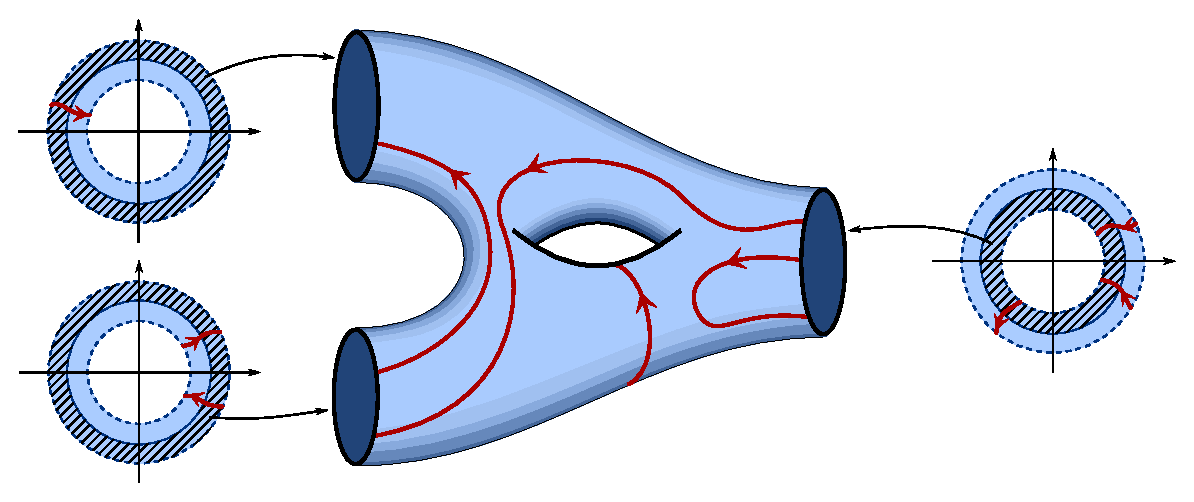
\includegraphics{pic02.eps}}}
  \put(0,0){
     \setlength{\unitlength}{.55pt}\put(-22,-8){
%     \put(136,224)   {$ \phi_\text{in} $}
%     \put(140, 22)   {$ \phi_\text{in} $}
%     \put(433,142)   {$ \phi_\text{out} $}
	 \put(295,190)   {$ {\scriptstyle Y} $}
	 \put(240,190)   {$ {\scriptstyle X} $}
	 \put(335,85)   {$ {\scriptstyle Z} $}
	 \put(390,105)   {$ {\scriptstyle Q} $}
     \put(510,180)   {$ O_{3} $}
     \put( 10,230)   {$ O_{1} $}
     \put( 10,110)   {$ O_{2} $}
     }\setlength{\unitlength}{1pt}}
  \end{picture}}
$$
\caption{A world-sheet $M$ with defect lines from $\,(O_1,O_2)\,$ to
$\,(O_{3})$.}
\label{fig:wsh-defect}
\end{figure}

With $\cat{B} = \LG$ an example of a morphism is given in Figure \ref{fig:wsh-defect}. The two-dimensional regions of $M$ are labelled with potentials and the defect lines are labelled with $1$-morphisms in $\LG$, that is, matrix factorisations. In the special case where we use a single label $W(x)$ for all regions, the labels $X,Y,Z,Q$ for the defect lines are all chosen from the set of $1$-morphisms $W \lto W$. The value of $\mathcal{Z}$ on $M$ is a $\nC$-linear map
\be\label{eq:value_of_bordism}
\mathcal{Z}(M): \mathcal{Z}(O_1) \otimes \mathcal{Z}(O_2) \lto \mathcal{Z}(O_3)\,.
\ee
We would like to discuss an additional property of the physicist's Landau-Ginzburg model which is not encoded into the data of the functor $\mathcal{Z}$. Namely, it is a consequence of the way the defect conditions $X,Y,Z,Q$ enter the partition function (see for example \cite[(3.16)]{laz}) that the vector spaces $\mathcal{Z}(O_i)$ and linear map $\mathcal{Z}(M)$ should depend continuously on the coefficients defining the defect conditions (TODO of course not). 

To represent this mathematically we might try to present $\mathcal{Z}(O_i)$ as a vector bundle over a scheme parametrising possible defect conditions and $\mathcal{Z}(M)$ as a morphism of these vector bundles. But there are some obstacles.
% \cite[(2.9)]{dkr1107.0495} 

Consider the incoming circle $O_2$ with two points marked $X,Y$. The construction gives
\be\label{eq:zo2orig}
\mathcal{Z}(O_2) := \Hom_{\LG(W,W)}( \Delta_W, Y^{\vee} \otimes X) \cong H^0 \Hom_{\nC[x,x']}( Y, X )
\ee
which is the vector space of $2$-morphisms $Y \lto X$ in $\LG(W,W)$. Now suppose that the defect conditions are made to depend on parameters 
\[
Y = Y(t_1,\ldots,t_r)\,, \qquad X = X(u_1,\ldots,u_s)
\]
which satisfy their own equations and cut out a parametrising scheme $\mathscr{M}_Y \times \mathscr{M}_X \subseteq \mathbb{A}^{r+s}$. The question is: what kind of global object $\mathcal{Z}(O_2)$ on $\mathscr{M}_Y \times \mathscr{M}_X$ is formed by the finite-dimensional vector spaces
\[
\mathcal{Z}(O_2)_{P,Q} := H^0 \Hom_{\nC[x,x']}( Y(P), X(Q) )
\]
as $P$ varies over $\mathscr{M}_Y$ and $Q$ over $\mathscr{M}_X$? The problem is that \emph{a priori} we have
\be\label{eq:cohom_sucks}
H^* \Hom_{\nC[x,x',t,u]}( Y(t), X(u) ) \Big\vert_{t=P, u=Q} \neq H^* \Hom_{\nC[x,x']}( Y(P), X(Q) )\,.
\ee
%This is a particular case of a general phenomenon: any complex of $\nC$-vector spaces $C$ is isomorphic in the derived category $\mathbb{D}(\nC)$ to $\bigoplus_n H^n(C)[n]$, but over a general ring, for instance the coordinate ring of $\mathscr{M}_Y \times \mathscr{M}_X$, this is not the case. 
This discrepancy suggests that we should take as our global object $\mathcal{Z}(O_2)$ the Hom complex itself, as an object in the derived category\footnote{Note that it is not enough to take the derived category of coherent sheaves, because the Hom complex is made up of non-finitely-generated modules over $\mathscr{M}_Y \times \mathscr{M}_X$.}
\be\label{eq:wuhe20}
\mathcal{Z}(O_2) := \Hom_{\nC[x,x',t,u]}( Y(t), X(u) ) \in \mathbb{D}( \operatorname{qcoh} \mathscr{M}_Y \times \mathscr{M}_X )\,.
\ee
An alternative (and we believe simpler) approach is to take $\cat{L}$ rather than $\LG$ as the input to the definition of the TFT. Before doing so, let us observe that in the situation where $X,Y$ do not depend on parameters, we may equivalently\footnote{This definition is not quite equivalent, because the displayed composite produces a complex of vector spaces quasi-isomorphic to $H^* \Hom(Y,X)$ rather than $H^0 \Hom(Y,X)$, but this is not important here.} define the vector space $\mathcal{Z}(O_2)$ from \eqref{eq:zo2orig} via the following composite in $\LG$:
\be\label{eq:composite_intro_o2}
\xymatrix@C+2pc{
0 \ar[r]^-X & W(x) - W(x') \ar[r]^-{Y^{\vee}} & 0
}\,.
\ee
Now let $\mathcal{Z}'$ be the TFT defined using the bicategory $\cat{L}$ as input. Then $\mathcal{Z}'(O_2)$ may likewise be computed by the composite \eqref{eq:composite_intro_o2} in $\cat{L}$, which is a $\nZ_2$-graded complex of vector spaces $Y^{\vee} \l X$ equipped with the action of a Clifford algebra. If $Y(t), X(u)$ are allowed to depend on parameters, the cut becomes a vector bundle
\be\label{eq:orynx}
\mathcal{Z}'(O_2) := Y^{\vee}(t) \l X(u)
\ee
over $\mathscr{M}_Y \times \mathscr{M}_X$ equipped with a differential and compatible Clifford action, such that
\be
Y^{\vee}(t) \l X(u) \Big\vert_{t=P,u=Q} \cong Y^{\vee}(P) \l X(Q)
\ee
for every point $(P,Q)$.

Since $\cat{L}$ and $\LG$ are equivalent, the two ways \eqref{eq:wuhe20},\eqref{eq:orynx} of reading the composite \eqref{eq:composite_intro_o2} must contain the same information. However, the fact that $\eqref{eq:orynx}$ is a finite rank vector bundle over $\mathscr{M}_Y \times \mathscr{M}_X$ while \eqref{eq:wuhe20} is a complex of (non-finitely generated) quasi-coherent sheaves explains why $\cat{L}$ is better suited to this kind of problem.

%We leave the details to the aforementioned sequel \cite{??}, but here is a simple example which already shows the nontriviality of viewing correlators as functionals of the moduli of the labels on defects. Consider the following bordism which is a morphism from the empty manifold $\emptyset$ to $O$, where $X$ denotes a matrix factorisation of $V(y) - W(x)$. The value of this diagram is an element
%\[
%\mathcal{Z}(M) \in \mathcal{Z}(O) \cong Jac(V)
%\]
%By virtue of the above discussion, we may think of $\mathcal{Z}(M)$ as a \emph{section} of the trivial vector bundle with fiber $Jac(V)$ over the scheme $\mathscr{M}(W,V)$ which parametrises $1$-morphisms from $W$ to $V$ in $\LG$. If this section is not identically zero, then $V$ is called a \emph{generalised orbifold} of $W$ \cite{??} and it is of great interest to know when this is the case. From what we have said, it is clear that this is essentially a question of the geometry of $\mathscr{M}(W,V)$.

TODO: discuss $A_\infty$ algebras. If we want to understand how minimal models vary with the coefficients, and where the jumps occur, we need an intermediate finite object over blah since minimal models only work well over a field.
